\documentclass[a4paper,11pt,fleqn]{scrartcl}%fleqn pour aligner les equations à gauche
\usepackage{../../Styles/Cours}


\newcommand{\chnum}{Chapitre 1}
\newcommand{\chtitle}{Mesurer le pH}
\newcommand{\dtype}{TP}

\begin{document}
\maketitle

Le pH renseigne sur l'acidité ou  la basicité d'une solution. Il dépend de la concentration en ions oxonium \ce{H3O+_{(aq)}} présents dans la solution.\\
\textbf{\textit{Problématique :} Le pH est une grandeur sans unité permettant d'apprécier le caractère acide ou basique d'une solution. Comment est donc définit le pH ?}\\
Pour répondre à cette question, nous allons préparer un ensemble de solutions de concentrations différentes et en mesurer le pH. les valeurs mesurées seront alors comparées aux valeurs théoriques.

\begin{figure}[h!]
    		\begin{minipage}{.4\linewidth}
    		\caption{\textbf{La définition du pH}}
        C'est au sein du laboratoire Carlsberg, chargé d'effectuer des recherches sur la fabrication de la bière, que le danois Soren SORENSEN introduit le notion de pH. Dès 1881, son prédécesseur à la direction du laboratoire, J. G. KJELDAHL, avait observé que l'activité de l'enzyme saccharase dépendait de la quantité des différents acides présents dans le milieu, mais aucune relation claire entre ces acides et l'activité enzymatique n'avait pu être établie. SORENSEN comprit que le facteur déterminant n'était pas la concentration en acides, mais la concentration en ions hydrogène \ce{H+} provenant de ces acides. C'est ainsi qu'il a été amené à définir le pH. Par la suite, cette définition a évolué en faisant intervenir les ions oxonium \ce{H3O+(aq)}, forme solvatée des ions hydrogène.
        \end{minipage}\hspace{1em}
        \begin{minipage}{.55\linewidth}
        \caption{\textbf{Complément scientifique}}
        L'eau distillée contient des molécules d'eau \ce{H2O(l)} mais également des ions oxonium \ce{H3O+(aq)} et des ions hydroxyde \ce{HO-(aq)} en quantités égales et très faibles : 
        [\ce{H3O+}] = \ce{HO-(aq)} = \SI{1E-7}{\mole\per\liter} à \SI{25}{\celsius}.\\
        
        \caption{\textbf{Matériel et solutions disponibles}}    
        \begin{itemize*}
        \item Solutions $S_1$ et $S_4$ d'acide chlorhydrique de concentration en ion oxonium [\ce{H3O+}] = \SI{1,0E-1}{\mole\per\liter} et [\ce{H3O+}] =\SI{1,0 E-4}{\mole\per\liter}.
        \setlength{\columnsep}{1cm}
        \begin{multicols}{2}
        \item pipettes jaugées de \SI{5.0}{mL} ; \SI{10}{mL} et \SI{20}{mL}
        \item propipette
        \item 3 fioles jaugées de \SI{50.0}{mL} avec bouchon
        \item 4 béchers
        \item pissette d'eau distillée
        \item pipette pasteur
        \item pH-mètre
        \item bandes de papier filtre
        \item tableur-grapheur ou edupython
        \item lunettes
        \end{multicols}
    \end{itemize*}
	\end{minipage}

    
\begin{minipage}{\linewidth}
\caption{\textbf{La solution d'acide chlorhydrique}}
Une solution d'acide chlorhydrique est une solution aqueuse contenant des ion oxonium \ce{H3O+(aq)} et des ions chlorure \ce{Cl-(aq)} en quantités identiques.\\
\textbf{Extrait de l'étiquette d'une solution concentrée d'acide chlorhydrique :}\\
\begin{tabular}{p{.65\textwidth} p{.35\textwidth}}
\textbf{Mentions de danger}&\\
\textbf{H290 :} peut être corrosif pour les métaux ; & \multirow{3}{*}{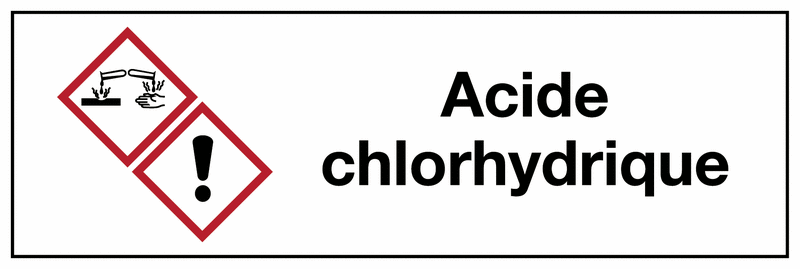
\includegraphics[scale=.2]{Ressources/Act1_Fig2.png}}\\
\textbf{H314 :} provoque des brûlures de la peau et des lésions oculaires graves ; &\\
\textbf{H335 :} peut irriter les voies respiratoires &\\
\end{tabular}
\end{minipage}
\end{figure}


\begin{table}[h]
	\begin{tabular}{|>{\centering}m{.12\textwidth} |>{\centering}m{.1\textwidth }|>{\centering}m{.1\textwidth} |>{\centering}m{.1\textwidth} |>{\centering}m{.1\textwidth} |>{\centering}m{.1\textwidth} |>{\centering}m{.1\textwidth} |>{\centering\arraybackslash}m{.1\textwidth} |}
	\hline
	Solution &$S_1$&$S_2$&$S_3$&$S_4$&$S_5$&$S_6$&Eau distillée\\
	\hline
	[\ce{H3O+}] (en \unit{\mole\per\liter})& \num{0,10} & \num{0,010} & \num{1,0E-3} & \num{1,0E-4} &\num{1,0E-5}& \num{1,0E-6} & \num{1,0E-7}\\
	\hline
	pH mesuré&&&&&&&\rule[1cm]{0cm}{0cm}\\
	\hline
	\end{tabular}
\end{table}
	
\section{Préparation des solutions}
\begin{enumerate}
	\item A partir du matériel disponible, proposer un protocole expérimental pour préparer trois solutions par dilution successives d'un facteur 10 à partir de la solution $S_1$ ou $S_4$.\\ \textit{Penser à bien préciser : les règles de sécurité / le nom du matériel et des espèces chimiques / les quantités utilisées.} \textcolor{gray!80!blue}{\textbf{ANA, COM}}
	\begin{center}
	\textbf{\textsc{Appel n°1}}
	\end{center}
	\item Mettre en œuvre le protocole de dilution. \textcolor{gray!80!blue}{\textbf{REA}}
\end{enumerate}
\section{Mesure du pH}
\begin{enumerate}[resume]
	\item \begin{enumerate}
		\item Lire la fiche méthode de l'utilisation d'un pH-mètre. \textcolor{gray!80!blue}{\textbf{APP}}
		\item Étalonner le pH-mètre. \textcolor{gray!80!blue}{\textbf{REA}}
		\item Mesurer le pH des 3 solutions précédentes et les 3 solutions d'un groupe ayant travaillé avec l'autre solution mère. Inscrire les résultats dans le tableau ci-dessus. \textcolor{gray!80!blue}{\textbf{REA}}
	\end{enumerate}
	\begin{center}
	\textbf{\textsc{Appel n°2}}
	\end{center}
\end{enumerate}
\section*{Exploitation des mesures}
\begin{enumerate}[resume]
	\item Compléter la première phrase du bilan. \textcolor{gray!80!blue}{\textbf{ANA}}
	\item Compléter les lignes 7, 10, 11 et 12 du programme Python fourni pour afficher les points représentant le pH en fonction de la concentration en ions oxonium. \textcolor{gray!80!blue}{\textbf{APP, ANA}}
	\item En déduire si le pH d'une solution est proportionnel à sa concentration en ions oxonium. Justifier. \textcolor{gray!80!blue}{\textbf{VAL}}
	\item Dans la deuxième phrase du bilan, indiquer comment varie le pH lorsque la concentration en ions oxonium de la solution diminue d'un facteur 10. \textcolor{gray!80!blue}{\textbf{ANA}}
	\item Tester alors les deux relations ci-dessous et en déduire laquelle convient pour définir le pH. Compléter alors la troisième phrase du bilan. \textcolor{gray!80!blue}{\textbf{ANA VAL}}
	\begin{center}
	\fbox{$pH = Log \frac{[H_3O^{+}]}{c^0}$} ou \fbox{$pH = -Log \frac{[H_3O^{+}]}{c^0}$}\\
	avec $c^0$ la concentration standard égale à $1~mol\cdot L^{-1}$
	\end{center}
	\begin{center}
	\textbf{\textsc{Appel n°3}}
	\end{center}
	\item Modéliser la courbe de la question 8. Pour cela, déplacer les lignes concernant le modèle (lignes 19 à 24) entre la ligne 13 et 14. A quoi sert la ligne 21 ? \textcolor{gray!80!blue}{\textbf{REA, ANA}}
\end{enumerate}

\begin{center}\fbox{\begin{minipage}{\linewidth}
\section{BILAN}
Plus la concentration en ions oxonium d'une solution est faible, plus le pH est .......................\\
Lorsque cette concentration est divisée par 10, le pH  ..................................\\
La relation entre pH est concentration en ions oxonium est :\\
\vspace{2em}

\end{minipage}}
\end{center}

\begin{figure}[t]
\begin{minipage}{.6\linewidth}
	\caption{\textbf{Code python}}
	\lstinputlisting[language = Python]{Ressources/TSPE_C01_AE1.py}
\end{minipage}
\end{figure}

\end{document}